\documentclass{article} % This command is used to set the type of document you are working on such as an article, book, or presenation

\usepackage{geometry} % This package allows the editing of the page layout
\usepackage{amsmath}  % This package allows the use of a large range of mathematical formula, commands, and symbols
\usepackage{graphicx}  % This package allows the importing of images
\usepackage{soul}
\usepackage{amsfonts}
\usepackage{dirtytalk}
\usepackage{tabto}
\usepackage{xcolor,colortbl, amssymb}
\usepackage{forest}
\usepackage[ruled, lined, linesnumbered, commentsnumbered, longend]{algorithm2e}

% https://www.messletters.com/en/big-text/

\newcommand{\question}[2][]{\begin{flushleft}
        \textbf{Problem #1}: \textit{#2}

\end{flushleft}}

\definecolor{Green}{rgb}{0, 1, 0}
\definecolor{Pink}{rgb}{1, .753, .796}

\newcommand{\sol}{\textbf{Solution}:} %Use if you want a boldface solution line
%\newcommand\tab[1][0.4cm]{\hspace*{#1}}
\newcommand{\maketitletwo}[2][]{\begin{center}
        \Large{\textbf{Homework #1}
            
            CMPSC 465} % Name of course here
        \vspace{5pt}
        
        \normalsize{Kinner Parikh  % Your name here
        
        \today}        % Change to due date if preferred
        \vspace{40pt}


        \newpage
        
\end{center}}
\begin{document}
    \maketitletwo[7]  % Optional argument is assignment number
    %Keep a blank space between maketitletwo and \question[1]

    \question[1]{}
    \begin{center}
        
        I worked with Sahil Kuwadia and Ethan Yeung
    
        I did not consult without anyone my group member
    
        I did not consult any non-class materials
    \end{center}
    
    \newpage

    \question[2]{}

    This statement is false. When $f$ is the maximum flow between $s$ and $t$, $f$ does not saturate every edge because in a given flow network, the maximum flow is simply the bottleneck of a given path. For example, given $G$:

    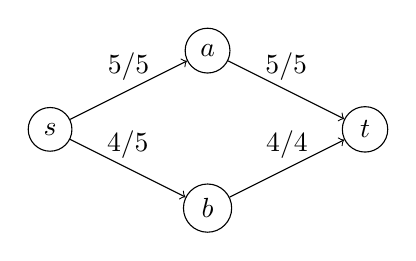
\begin{tikzpicture}[scale=1,auto=center]

        \node[circle, draw] (s) at (0, 1) {$s$};
        \node[circle, draw] (a) at (2, 2) {$a$};
        \node[circle, draw] (b) at (2, 0) {$b$};
        \node[circle, draw] (t) at (4, 1) {$t$};

        %\draw[->] (s) tonode[above]{0/10} (a);
        % \draw[->] (s) tonode[above]{5/10} (c);
        % \draw[->] (a) tonode[above]{5/25} (b);
        % \draw[->] (c) tonode[above]{5/15} (d);
        % \draw[->] (d) tonode[above]{5/5} (a);
        %\draw[->] (d) tonode[above]{0/10} (t);
        % \draw[->] (b) tonode[above]{5/10} (t);
        \draw[->] (s) tonode[above]{5/5} (a);
        \draw[->] (s) tonode[above]{4/5} (b);
        \draw[->] (a) tonode[above]{5/5} (t);
        \draw[->] (b) tonode[above]{4/4} (t);

    \end{tikzpicture}

    We can see that the maximum flow from $s$ to $t$ is 9 because of the bottleneck edge $(b, t)$. This means on the path that follows $(s, b, t)$, not every edge is saturated. So this counterexample proves that not every edge out of $s$ is saturated.

    \newpage

    \question[3]{}

    We can find the solution to this problem by creating a flow network graph. We can first create a node for every patient ($p_i$ where $i \in [1,n]$) and every hospital ($h_j$ where $j \in [1,k]$) in the area. Then, create an edge from every patient to every hospital ($p_i, h_j$), and set the maximum capacity of that edge to 1 if and only if $p_i$ can get to $h_j$ within the half hour time limit, else set the capacity of that edge to 0. Now that we established this flow network, we have to create source and sink nodes to be able to find optimal paths for patients to be admitted to hospitals. We can create a source node $s$ that has edges defined as ($s, p_i$) of capacity 1. We can create a sink node $t$ that has edges ($h_j, t$) such that every hospital node is connected to the sink of capacity $\lceil n/k \rceil$. This sets up the initial flow graph.

    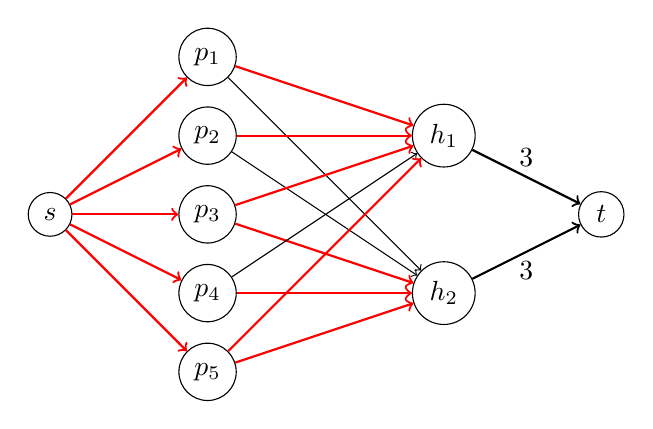
\begin{tikzpicture}[scale=1,auto=center]

        \node[circle, draw] (s) at (1, 2) {$s$};
        \node[circle, draw] (p1) at (3, 4) {$p_1$};
        \node[circle, draw] (p2) at (3, 3) {$p_2$};
        \node[circle, draw] (p3) at (3, 2) {$p_3$};
        \node[circle, draw] (p4) at (3, 1) {$p_4$};
        \node[circle, draw] (p5) at (3, 0) {$p_5$};
        \node[circle, draw] (h1) at (6, 3) {$h_1$};
        \node[circle, draw] (h2) at (6, 1) {$h_2$};
        \node[circle, draw] (x) at (8, 2) {$t$};

        \draw[->, red, thick] (s) tonode[above]{} (p1);
        \draw[->, red, thick] (s) tonode[above]{} (p2);
        \draw[->, red, thick] (s) tonode[above]{} (p3);
        \draw[->, red, thick] (s) tonode[above]{} (p4);
        \draw[->, red, thick] (s) tonode[above]{} (p5);
        \draw[->, red, thick] (p1) tonode[above]{} (h1);
        \draw[->] (p1) tonode[above]{} (h2);
        \draw[->, red, thick] (p2) tonode[above]{} (h1);
        \draw[->] (p2) tonode[above]{} (h2);
        \draw[->, red, thick] (p3) tonode[above]{} (h1);
        \draw[->, red, thick] (p3) tonode[above]{} (h2);
        \draw[->] (p4) tonode[above]{} (h1);
        \draw[->, red, thick] (p4) tonode[above]{} (h2);
        \draw[->, red, thick] (p5) tonode[above]{} (h1);
        \draw[->, red, thick] (p5) tonode[above]{} (h2);
        \draw[->, thick] (h1) tonode[above]{3} (x);
        \draw[->, thick] (h2) tonode[below]{3} (x);
    \end{tikzpicture}

    In this example, assume that all red edges have a capacity of 1, thin edges without a number have a capacity of 0, and the two edges connecting $h_1$ and $h_2$ to $t$ have a capacity of $\lceil 5/2 \rceil = 3$. We can observe that all patients have an edge to all hospitals. Having created this graph, we can simply apply the Ford-Fulkerson algorithm to find the maximum possible flow from $s$ to $t$. We know that if the maximum flow from $s$ to $t$ is $n$, then every single person can be brought to a hospital. 

    \vspace{5pt}

    Runtime: To find the runtime, we must determine the runtime of the Ford-Fulkerson algorithm. We know that the algorithm is $O(C \cdot |E|)$, where $C$ is the sum of capacities leaving the source node, which is $n$ in this case. Since there is an edge from every patient to every hospital, $|E| = n \cdot k$. Putting all the steps together, we see that initialization takes $\Theta(n \cdot k + n + k)$ for creating all the edges of the graph. So $\Theta(n \cdot k + n + k) + O(n \cdot n \cdot k) = O(n^2k)$, which is polynomial time.

    \newpage

    \question[4]{Prove that if $f_1$ and $f_2$ are valid, then $\alpha f_1 + (1-\alpha)f_2, \forall \alpha \in [0, 1]$ is a valid flow}

    We can say that the maximum flow from $u$ to $v$ can be defined by the function $mFlow(u, v)$.

    \vspace{5pt}

    So, assuming that $f_1$ and $f_2$ are valid flows from $u$ to $v$, then: 
    
    \underline{Property 1:} $f_1 \leq mFlow(u, v)$ and $f_2 \leq mFlow(u, v)$

    \vspace{5pt}

    To prove that flows of a network produce a convex set, we must show that:

    $\alpha f_1 + (1-\alpha)f_2 \leq mFlow(u, v), \forall \alpha \in [0, 1]$.

    \vspace{5pt}

    Expanding the left side:

    $\alpha f_1 + (1-\alpha)f_2 \leq \alpha \cdot mFlow(u, v) + (1 - \alpha) \cdot mFlow(u, v)$ [Property 1]

    \hspace{2.5cm}$\leq (\alpha + 1 - \alpha) \cdot mFlow(u, v)$

    \hspace{2.5cm}$\leq 1 \cdot mFlow(u, v)$

    Thus, 

    $\alpha f_1 + (1-\alpha)f_2 \leq mFlow(u, v)$ proving that flows from a network form a convex set.
    

    
\end{document}
